\documentclass{ximera}
\usepackage{sagetex}
%% handout
%% space
%% newpage
%% numbers
%% nooutcomes

%% You can put user macros here
%% However, you cannot make new environments

\graphicspath{{./}{module1Activity/}{module2Activity/}{module3Activity/}}

\usepackage{sagetex}
\usepackage{tikz}
\usepackage{hyperref}
\usepackage{tkz-euclide}
\usetkzobj{all}
\pgfplotsset{compat=1.7} % prevents compile error.

\tikzstyle geometryDiagrams=[ultra thick,color=blue!50!black]
 %% we can turn off input when making a master document

\outcome{}
\author{Darryl Chamberlain Jr.}
 
\title{Objective 2 - Graph}

\begin{document}
\begin{abstract}
Identify the graph of a radical function.
\end{abstract}
\maketitle

\textit{Note: No section in the textbook directly talks about how to graph radical functions.}

%%%%%%%%%%%%%%%%%%%%%
%%%  Objective 2  %%%
%%%%%%%%%%%%%%%%%%%%%

You can print out \href{http://people.clas.ufl.edu/dchamberlain31/files/M5-Objective-2-Graph-Radical-Functions.pdf}{these notes} to follow along with the video below and keep notes to organize your thoughts.

\youtube{dX-mB0MlWvQ}

I also suggest visiting \href{https://www.desmos.com/calculator/sa2j9mats1}{this Desmos page} to see how various numbers affect radical functions. Focus on what changing $h$ and $k$ does to each type of radical function.

% TWO STATIC GRAPHS OF SQUARE ROOTS AND TWO STATIC GRAPHS OF CUBE ROOTS.

% Q1
\begin{question}
Write the equation of the function graphed below. Assume $a = 1$ or $a = -1$.  

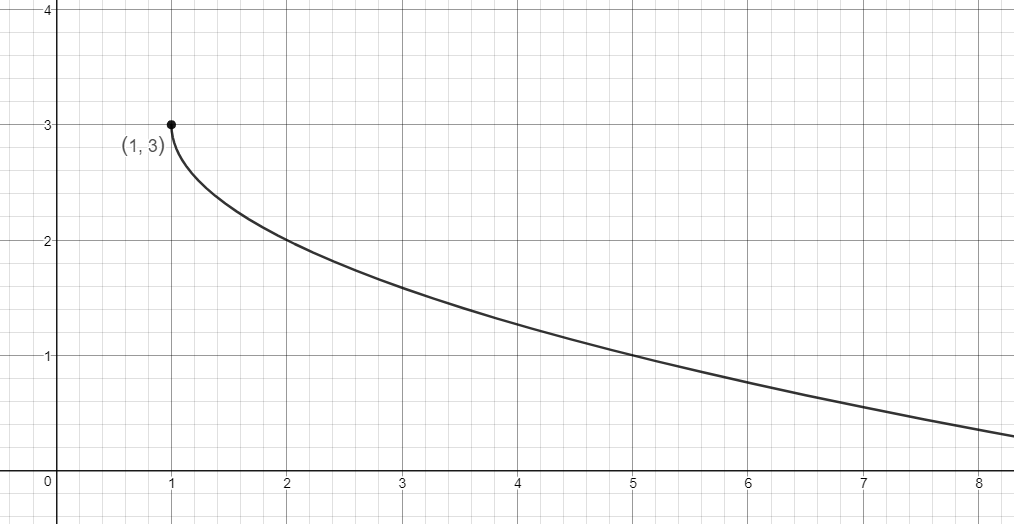
\includegraphics{graphRadicalQ1.png}

$f(x) = \answer{-1} \sqrt{\answer{x-1}}$ $+ \answer{3}$ 

\end{question}

% Q6
\begin{question}
Write the equation of the function graphed below. Assume $a = 1$ or $a = -1$. \\

\textit{Hint: Be sure to remove the decimal. For example, if $x$ is shifting by $0.75$ to the right, then standard form would be $4x-3$ rather than $x-0.75$.}

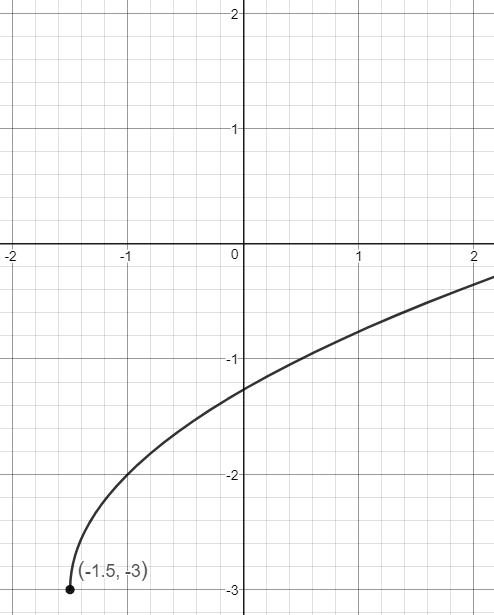
\includegraphics{graphRadicalQ2.png}

$f(x) = \answer{1}$ $\sqrt{\answer{2x+3}}$ $+ \answer{-3}$

\end{question}

% Q7
\begin{question}
Write the equation of the function graphed below. 

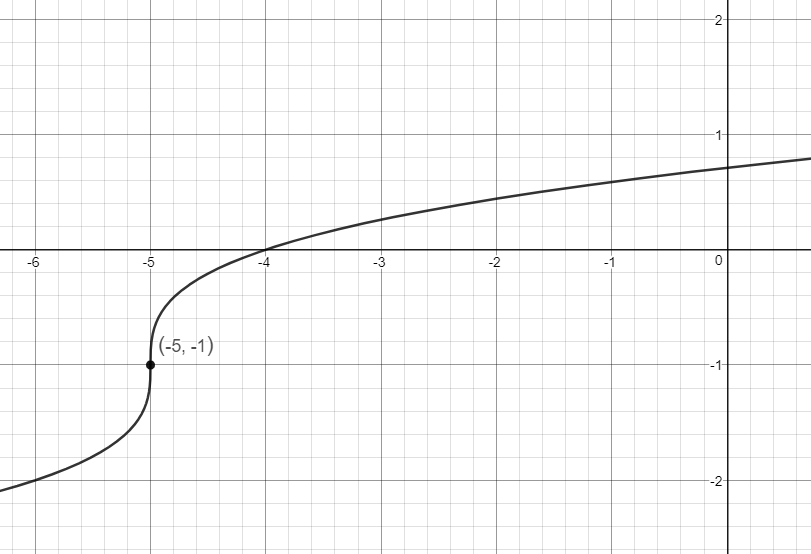
\includegraphics{graphRadicalQ3.png}

$f(x) = \answer{1}$ $\sqrt[3]{\answer{x+5}}$ $+ \answer{-1}$ 

\end{question}

% Q8
\begin{question}
Write the equation of the function graphed below. \textit{Hint: Be sure to remove the decimal. For example, if $x$ is shifting by $0.75$ to the right, then standard form would be $4x-3$ rather than $x-0.75$.}

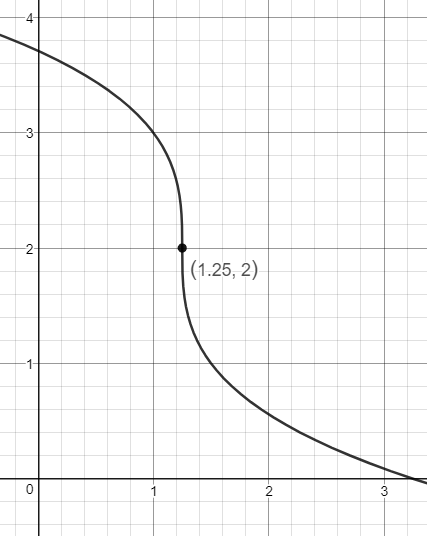
\includegraphics{graphRadicalQ4.png}

$f(x) = \answer{-1} \sqrt[3]{\answer{4x-5}}$ $+ \answer{2}$

\end{question}

\end{document}
